\documentclass{standalone}
\usepackage{tikz}
\usetikzlibrary{arrows}
\usetikzlibrary{arrows.meta}
\usetikzlibrary{bending}
\usetikzlibrary{shadows}
\usetikzlibrary{positioning}
\usetikzlibrary{calc}
\usetikzlibrary{decorations.text}
\usetikzlibrary{backgrounds}
\usepackage[hidelinks]{hyperref}

\begin{document}
\scalebox{1.2}{
  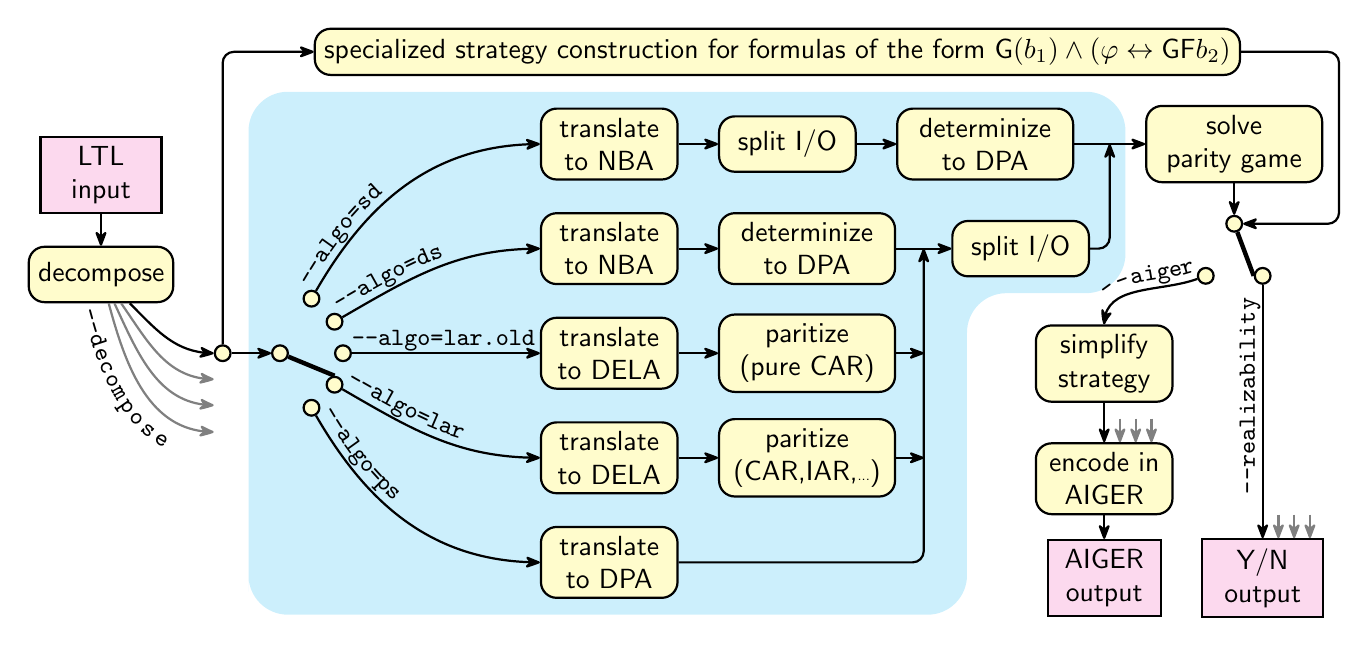
\begin{tikzpicture}[thick,font=\sffamily,>={Stealth[round,bend]},
                      node distance=4mm and 5mm,
                      data/.style={text width=1.3cm,minimum height=2em,align=center,draw,fill=magenta!15},
                      wproc/.style={fill=yellow!20,align=center,draw,rounded corners=2mm},
                      proc/.style={wproc,text width=1.5cm,minimum height=2em},
                      lproc/.style={proc,text width=2cm},
                      choice/.style={circle,fill=yellow!20,inner sep=0,minimum size=2mm,draw},
                      algoopt/.style={postaction={decorate,decoration={text along path, raise=1mm,text={|\ttfamily\small|#1}}}},
                      algooptd/.style={postaction={decorate,decoration={text along path, raise=-1em,text={|\ttfamily\small|#1}}}},
                      outopt/.style={postaction={decorate,decoration={text along path, text align=right,raise=1mm,text={|\ttfamily\small|#1}}}},
                      ]
    \node[proc] (transSD) {translate to NBA};
    \node[proc,right=of transSD] (splitSD) {split I/O};
    \node[lproc,right=of splitSD] (detSD) {determinize to DPA};
    \draw[->] (transSD) edge (splitSD)
              (splitSD) edge (detSD);
    \node[proc,below=of transSD] (transDS) {translate to NBA};
    \node[lproc,right=of transDS] (detDS) {determinize to DPA};
    \node[proc,right=of detDS,xshift=2mm] (splitDS) {split I/O};
    \draw[->] (transDS) edge (detDS)
              (detDS) edge coordinate(middetsplit) (splitDS);
    \node[proc,below=of transDS] (transLARold) {translate to DELA};
    \node[lproc,right=of transLARold] (paritizeLARold) {paritize (pure CAR)};
    \draw[->] (transLARold) edge (paritizeLARold)
              (paritizeLARold) edge (middetsplit |- paritizeLARold);
    \node[proc,below=of transLARold] (transLAR) {translate to DELA};
    \node[lproc,right=of transLAR] (paritizeLAR) {paritize (CAR,IAR,{\tiny ...})};
    \draw[->] (transLAR) edge (paritizeLAR)
              (paritizeLAR) edge (middetsplit |- paritizeLAR);
    \node[proc,below=of transLAR] (transPS) {translate to DPA};
    \draw[rounded corners,->] (transPS) -| (middetsplit);
    \coordinate (choicecenter) at ($(current bounding box.west) - (3.3cm,0)$);
    \path[draw] (choicecenter) node[choice](algoin){}
          +(60:8mm) node[choice](algosd){}
          +(30:8mm) node[choice](algods){}
          +(0:8mm) node[choice](algolarold){}
          +(-30:8mm) node[choice](algolar){}
          +(-60:8mm) node[choice](algops){};

    \draw[->,algoopt={-{}-algo=sd}] (algosd) to[out=60,in=180] (transSD);
    \draw[->,algoopt={-{}-algo=ds}] (algods) to[out=30,in=180] (transDS);
    \draw[->,algoopt={-{}-algo=lar.old}] (algolarold) -- (transLARold);
    \draw[->,algoopt={-{}-algo=lar}] (algolar) to[out=-30,in=180] (transLAR);
    \draw[->,algoopt={-{}-algo=ps}] (algops) to[out=-60,in=180] (transPS);
    \draw[ultra thick] (algoin) -- (algolar.north);

    \node[choice,left=of algoin] (bypassin) {};
    \node[proc,left=of bypassin,yshift=1cm,text width=1.6cm] (decomp) {decompose};
    \node[data,above=of decomp] (input) {LTL input};
    \draw[->] (input) -- (decomp);
    \draw[->] (decomp) to[out=-45,in=180] (bypassin);
    \draw[->,gray] (decomp) to[out=-55,in=180] ($(bypassin.west)+(0,-0.33)$);
    \draw[->,gray] (decomp) to[out=-65,in=180] ($(bypassin.west)+(0,-0.66)$);
    \draw[->,gray,algooptd={-{}-decompose}] (decomp) to[out=-75,in=180] ($(bypassin.west)+(0,-1)$);
    \draw[->] (bypassin) -- (algoin);

    \node[lproc, right=of detSD, xshift=4mm] (solve) {solve\linebreak parity game};

    \node[below=of solve,choice] (reachoice) {};
    \node[below right=of reachoice,choice,xshift=-3mm,yshift=-1mm] (realize) {};
    \node[below left=of reachoice,choice,xshift=3mm,yshift=-1mm] (aiger) {};
    \draw[ultra thick] (reachoice) -- (realize.west);
    \draw[->] (solve) -- (reachoice);


    \node[data] (yesno) at ($(transPS -| realize)+(0,-2mm)$) {Y/N output};
    \node[data, text width=1.2cm, left=of yesno] (output) {AIGER output};
    \node[proc, above=of output,yshift=-1mm] (encode) {encode in AIGER};
    \node[proc, above=of encode,yshift=+1mm] (minimize) {simplify\linebreak strategy};

    \draw[->] (detSD) -- coordinate(middetsolve) (solve);
    \draw[rounded corners,->] (splitDS) -| (middetsolve);

    \draw[<-,outopt={-{}-aiger}] (minimize) to[out=90,in=-160]  (aiger);
    \draw[->] (minimize) -- (encode);
    \draw[gray,->] ($(encode.north)+(2mm,3mm)$) -- ($(encode.north)+(2mm,0)$);
    \draw[gray,->] ($(encode.north)+(4mm,3mm)$) -- ($(encode.north)+(4mm,0)$);
    \draw[gray,->] ($(encode.north)+(6mm,3mm)$) -- ($(encode.north)+(6mm,0)$);
    \draw[<-,outopt={-{}-realizability~}] (yesno) -- (realize);
    \draw[gray,->] ($(yesno.north)+(2mm,3mm)$) -- ($(yesno.north)+(2mm,0)$);
    \draw[gray,->] ($(yesno.north)+(4mm,3mm)$) -- ($(yesno.north)+(4mm,0)$);
    \draw[gray,->] ($(yesno.north)+(6mm,3mm)$) -- ($(yesno.north)+(6mm,0)$);

    %\draw[->] (solve) -- (encode);
    \draw[->] (encode) -- (output);

  \begin{scope}[on background layer,overlay]
    \fill[cyan!20,rounded corners=5mm]
    ($(algoin |- transPS.south)+(-.4,-.2)$) |-
    ($(detSD.north -| middetsolve)+(.2,.2)$) |-
    ($(splitDS.south west)+(.2,-.2)$) |- cycle;
  \end{scope}

  \coordinate (solveright) at ($(solve.east)+(2mm,0)$);
  \path (bypassin) -- coordinate(medblue) (solveright);
  \node[wproc,above,xshift=-1mm,yshift=4mm] (bypass) at (medblue |- detSD.north) {specialized strategy construction for formulas of the form $\mathsf{G}(b_1) \land (\varphi \leftrightarrow \mathsf{G}\mathsf{F} b_2)$};
  \draw[rounded corners,->] (bypassin) |- (bypass);
  \draw[rounded corners,->] (bypass) -| (solveright) |- (reachoice);
  \end{tikzpicture}}
\end{document}
